\renewcommand{\kapitelautor}{Autor: Felix Zwickelstorfer}
\section{Screens}\label{sec:screens}

\renewcommand{\kapitelautor}{Autor: Felix Zwickelstorfer}

In Forty-Five werden grafische Elemente in onj als Teil eines Screens definiert.
Dabei sind sich stark voneinander unterscheidende Elemente ein eigener Screen, wie \zB der Kampf, die Karte oder der Shop.
Ein Screen besteht dabei aus einem Root-Element, in dem Child-Elemente sind.
Zusätzlich dazu hat jeder Screen einen Screen-Controller, welcher für die Verwaltung des Screens zuständig ist und komplexere Aufgaben in diesem durchführt.

Im Folgenden werden die einzelnen Bestandteile genauer erklärt und als Beispiel ein Teil des HealOrMaxHPScreen genommen.
Bei diesem kann sich der Spieler entweder heilen oder seine maximale Lebensanzahl erhöhen.
\begin{figure}[H]
    \centering
    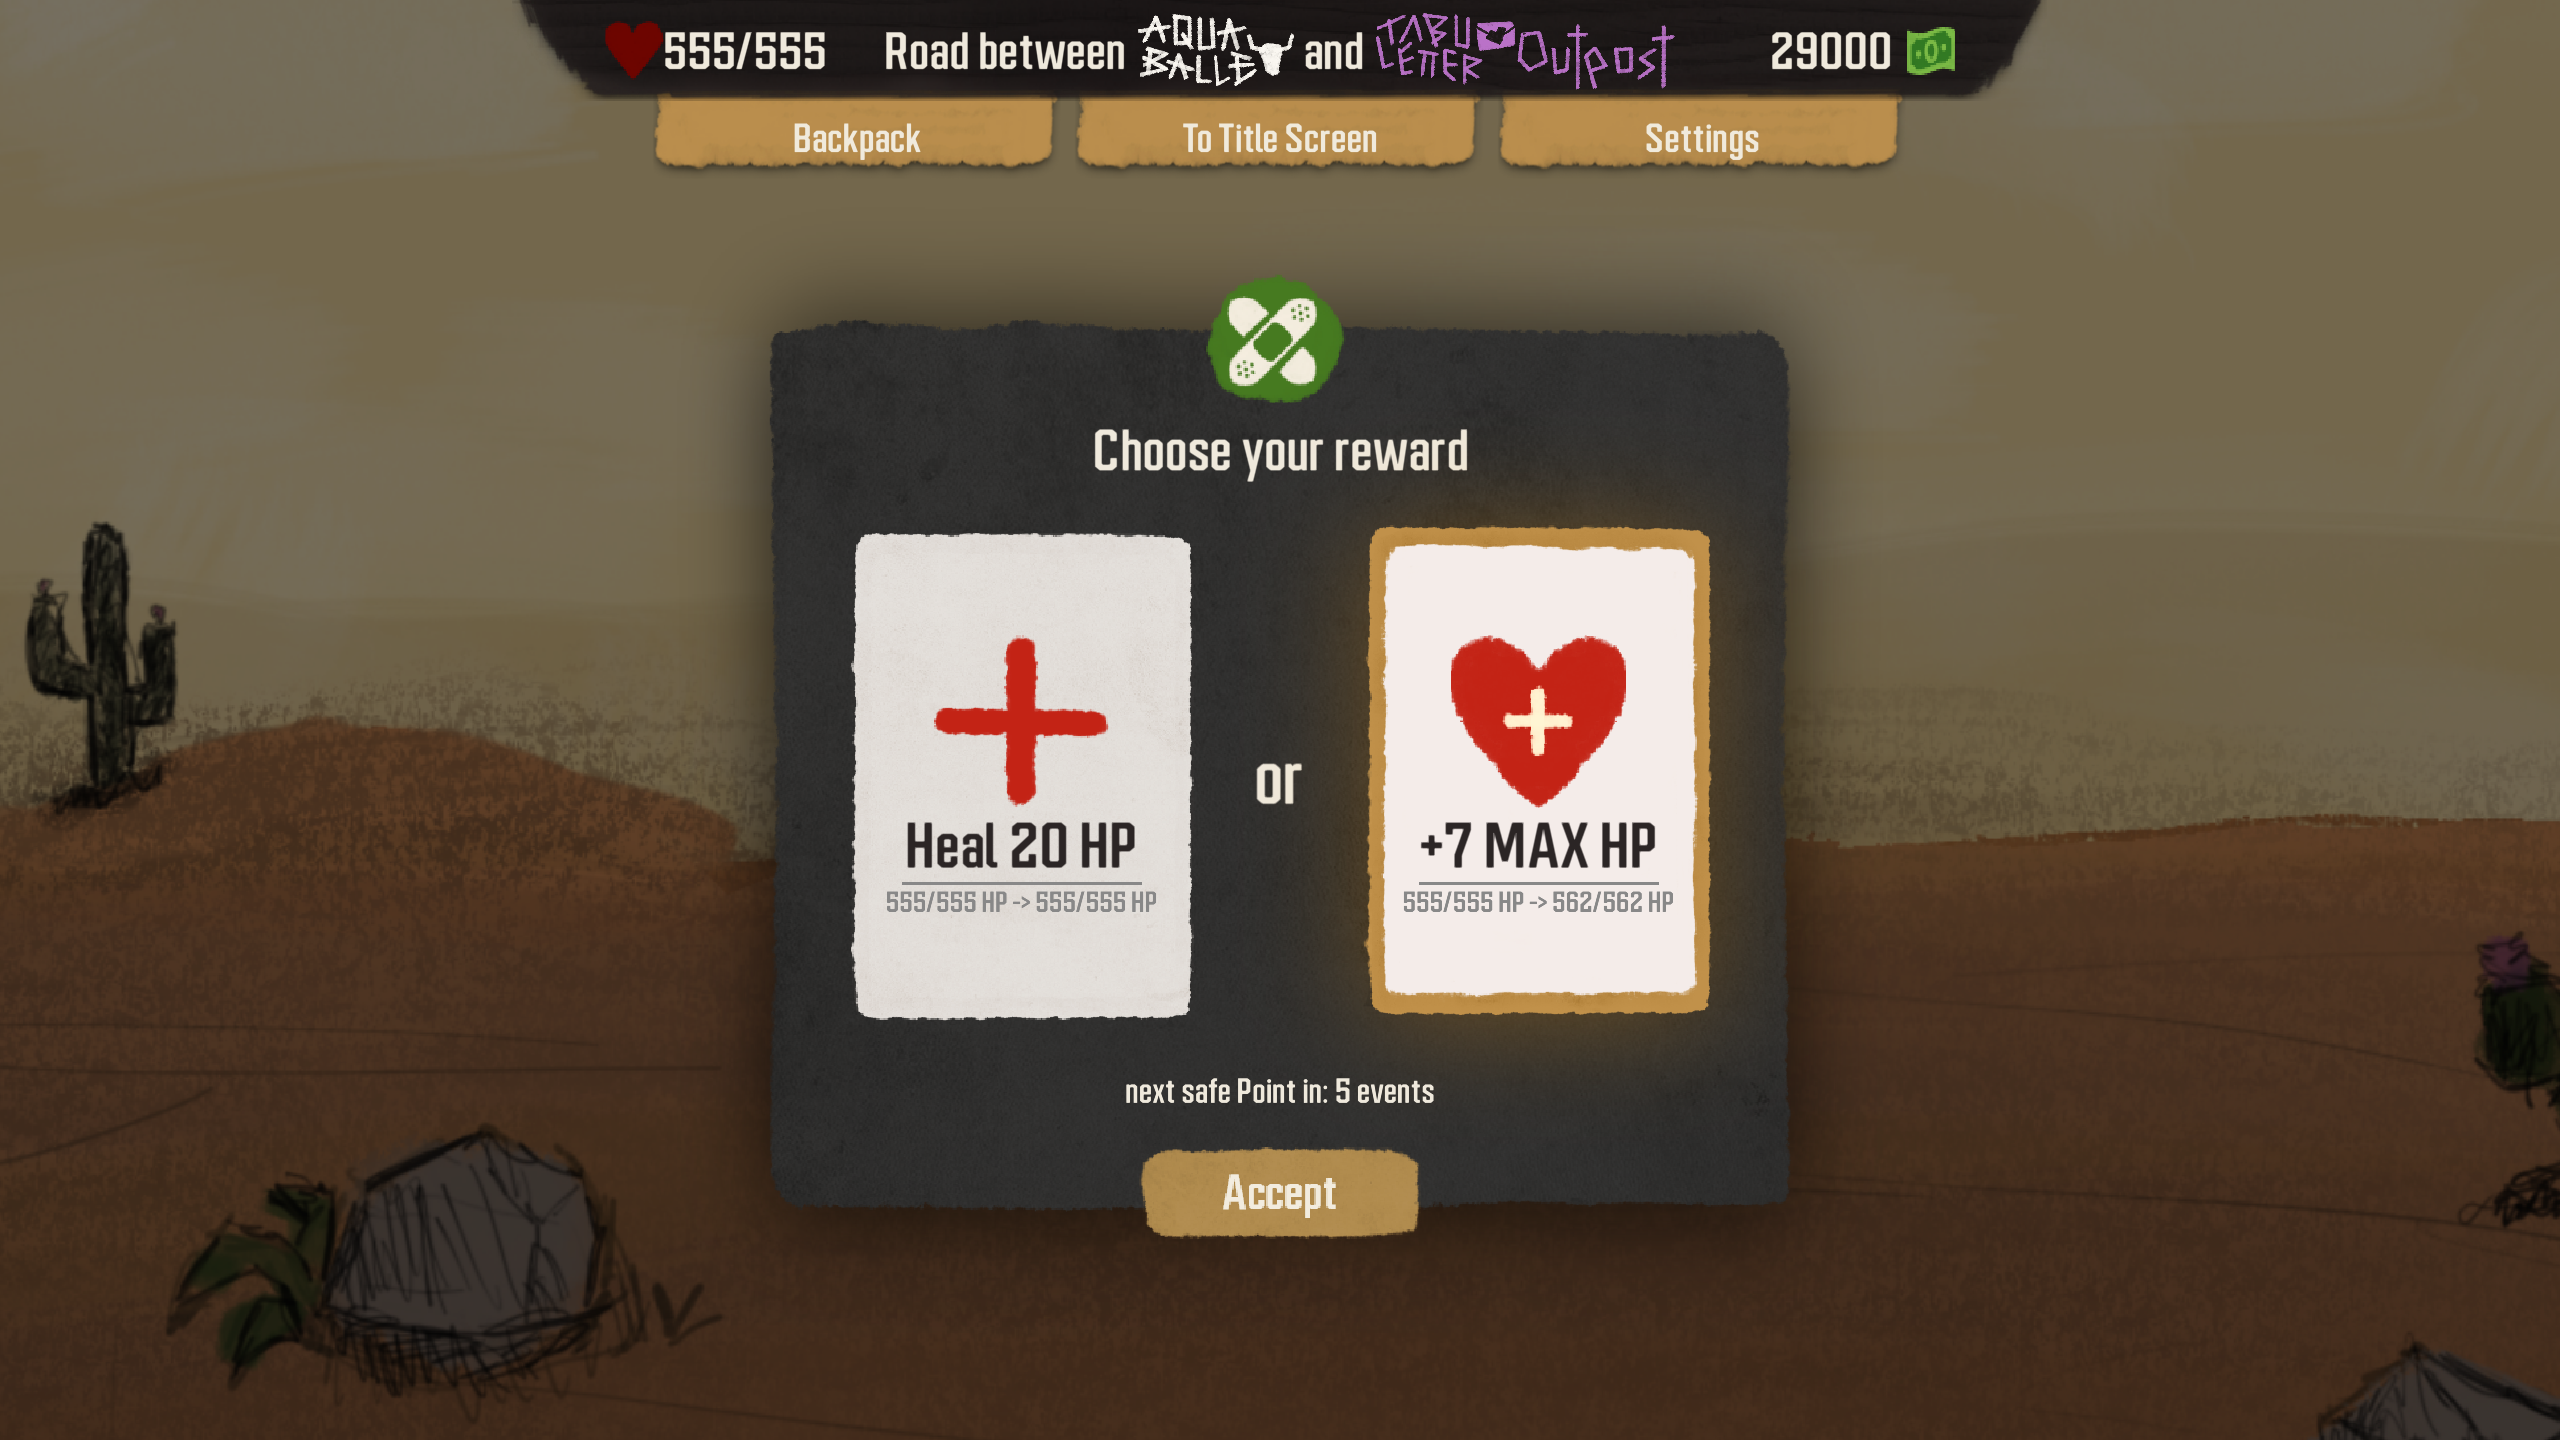
\includegraphics[width=1.0\textwidth]{healormaxhpevent.png}
    \caption{Screenshot des HealOrMaxHP-Screens}
\end{figure}

\renewcommand{\kapitelautor}{Autor: Felix Zwickelstorfer}
\subsection{Widgets}\label{sec:widgets}
\renewcommand{\kapitelautor}{Autor: Felix Zwickelstorfer}

Ein Widget beschreibt jedes Element, welches auf einem Screen sichtbar ist.
Die meisten werden von jedem Screen gebraucht, wie \zB das Box-Widget, welches eine Flexbox darstellt.
Es gibt allerdings Elemente, die wegen ihrer Komplexität oder Dynamik nicht als eine Schachtelung von anderen Elementen dargestellt werden können.
Diese werden zu ihrem eigenen Widget, welches vom Controller verwaltet wird, wie \zB die Map.
Alle Widgets sind definiert in \inlineCode{assets/onjschemas/screen.onjschema}.
Als Beispiel folgt nun das grüne Icon in der Mitte:




\begin{codeBlock}{onj}{Beispiel: Definition eines Images und der Statusbar aus heal\_or\_max\_screen.onj}
    $Image {
        name: "heal_icon",
        textureName: "map_node_heal",
        zIndex: 160,
        scaleX: 1.0,
        scaleY: 1.0,
        styles: [
            {
                positionType: positionType.absolute,
                positionTop: 19#percent,
                positionLeft: 47.15#percent,
            }
        ],
    }
\end{codeBlock}



Es gibt diverse Parameter, die nur für Images gelten, während andere "widget shared keys" sind, \dah, dass sie für alle gewöhnlichen Widgets verfügbar sind.
Diese beinhalten in dem oben angeführten Beispiel den name und die styles, welche auch die am häufigsten Verwendeten sind.
Es gibt allerdings auch die keys "behaviours" und "dragAndDrop", welche das Verhalten beim Interagieren des Benutzers definieren.

\renewcommand{\kapitelautor}{Autor: Felix Zwickelstorfer}
\subsubsection{Templates}\label{sec:templates}
\renewcommand{\kapitelautor}{Autor: Felix Zwickelstorfer}

Templates sind ein weiterer wichtiger Part von Widgets, da sie das dynamische Erstellen von Elementen im Code erleichtern.
